\subsubsection*{Analysis}
\begin{tabular}{@{}l l}
\textbf{Scope}:&The AuctionHouse\textsuperscript{TM} automated administration system\\
\textbf{Level}:&User goal\\
\textbf{Primary Actor}:&Purchasing Agent\\
\textbf{Stakeholders and Interests}:&\begin{tabular}[t]{@{}l}
	Purchasing Agent: wants to register an item easily and quickly.\\
	Auctioneer: wants the item to be registered for an upcoming auction.\\
	Seller: wants his goods to be visible to potential buyers.\\
	Buyer: wants to be notified if they are currently have a search request on this item.\end{tabular}\\
\textbf{Preconditions}:&Purchasing agent is identified and authenticated.\\
\textbf{Postconditions}:&\begin{tabular}[t]{@{}l}
	The item has been registered to the system, or a failure was returned.\\
	The product has been registered for an upcoming auction.\\
	The item is visible for potential buyers and the otherwise authorized.\\
	Buyers with a search request on this item are notified of the addition.
	\end{tabular}\\
\textbf{Special requirements}:&A list of categories and a list of future auction dates needs to available in the system\\
\textbf{Frequency of occurence}:& \begin{tabular}[t]{@{}l}Depedent on the amount of sellers and auctions per month.\\Since there is 1 auction per month. If we expect about 30 sellers, then there\\are 30 occurences per month, so about 1 per day.\end{tabular}
\end{tabular}\\\\
\textsl{Main Success Scenario}
\begin{enumerate}[noitemsep]
	\item The user starts the `add item' transaction with the system, having all parameters of the item to be added ready.
	\item The system provides the user with a list of categories to choose from, and a list of future planned aution dates.
	\item The user provides all necessary parameters and chooses a category for the item, and an auction date. The parameters to provide are:
	\begin{itemize}[noitemsep]
		\item The amount of the item available
		\item The type of item
		\item A description
		\item If the item possesses any antiquarian value
		\item A minimum price decided by the owner
		\item The date when brought in
		\item Name and address of the owner plus identification
		\item Planned auction date
		\item Distinguishing features
	\end{itemize}
	\item The system adds the item with all provided parameters to the list and generates an Item ID unique to the item.
	\item The system checks if there are any search requests looking for this specific item, and notifies the buyers that issued the request that the item is now available.
	\item The system returns to the user with a confirmation message containing the generated item ID.
\end{enumerate}
\textsl{Extensions}
\begin{itemize}[noitemsep]
	\item If the provided parameters are provided, the system does not continue to add the item, but asks the user to provide the remaining information.
	\item If an identical item is already registered in the system, the system terminates the transaction, leaving the system state unchanged.
	\item If the system fails to add the item to the list (perhaps due to internal/system limitations), the process is aborted and the transaction is terminated, rolling back the system state to the most recent stable (when no such problems occured) version.
\end{itemize}
\textsl{System Sequence Diagram}
\begin{figure}[H]
	\centering
	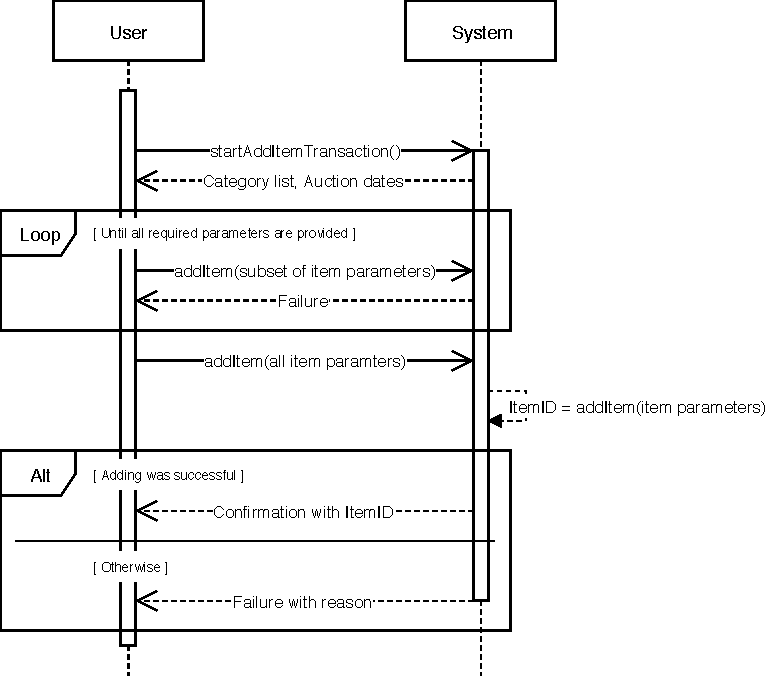
\includegraphics[scale=1]{uml/SD-bb-create.pdf}
	\caption*{Interactions displayed in a System Sequence Diagram defined by the MSS and its extensions in blackbox format}
\end{figure}